% ****** Start of file apssamp.tex ******
%
%   This file is part of the APS files in the REVTeX 4.1 distribution.
%   Version 4.1r of REVTeX, August 2010
%
%   Copyright (c) 2009, 2010 The American Physical Society.
%
%   See the REVTeX 4 README file for restrictions and more information.
%
% TeX'ing this file requires that you have AMS-LaTeX 2.0 installed
% as well as the rest of the prerequisites for REVTeX 4.1
%
% See the REVTeX 4 README file
% It also requires running BibTeX. The commands are as follows:
%
%  1)  latex apssamp.tex
%  2)  bibtex apssamp
%  3)  latex apssamp.tex
%  4)  latex apssamp.tex
%
\documentclass[%
 reprint,
superscriptaddress,
%groupedaddress,
%unsortedaddress,
%runinaddress,
%frontmatterverbose,
%preprint,
%showpacs,preprintnumbers,
%nofootinbib,
%nobibnotes,
%bibnotes,
 amsmath,amssymb,
 aps,
%pra,
%prb,
%rmp,
%prstab,
%prstper,
%floatfix,
]{revtex4-1}
\usepackage{color}
\usepackage{hyperref}
\usepackage{float}
\usepackage{textcomp}
\usepackage{epsfig}
\usepackage{epstopdf}
\usepackage{natbib}
\usepackage{multirow}

%\usepackage{graphix}
\usepackage{graphicx}% Include figure files
\usepackage{dcolumn}% Align table columns on decimal point
\usepackage{bm}% bold math
%\usepackage{hyperref}% add hypertext capabilities
%\usepackage[mathlines]{lineno}% Enable numbering of text and display math
%\linenumbers\relax % Commence numbering lines

\begin{document}
%\bibliographystyle{plain}
\preprint{APS/123-QED}

\title{Room temperature tunable gate frequency InGaAs/InP single-photon detector based on ADC samping method   }% Force line breaks with \\
%\thanks{A footnote to the article title}%
\author{Huan Chen}
\affiliation{Department of Physics, National University of Defense Technology, Changsha, 410073 People’s Republic of China}%
 \author{Musheng Jiang}%
 \affiliation{Zhengzhou Information Science and Technology Institute, Zhengzhou 450004, China }
  \author{Shihai Sun}
  \affiliation{Department of Physics, National University of Defense Technology, Changsha, 410073 People’s Republic of China}%
   \author{Guangzhao Tang}
   \affiliation{Department of Physics, National University of Defense Technology, Changsha, 410073 People’s Republic of China}%
    \author{Linmei Liang}%
    \email{nmliang@nudt.edu.cn}
    \affiliation{Department of Physics, National University of Defense Technology, Changsha, 410073 People’s Republic of China}%
    \affiliation{State Key Laboratory of High Performance Computing, National University of Defense Technology, Changsha 410073,People's Republic of China}

\begin{abstract}
The available high speed InGaAs/InP-based single-photon avalanche detectors(SPAD) are normally worked at fixed gate repetition frequency. Here, we present a high speed InGaAs/InP-based SPAD working at telecom wavelength of 1.55\textmu m with tunable gate frequency from 900MHz to 1100MHz. In the SPAD, a high speed, 14 bits resolution analog to digital convertor (ADC) is used to sample one voltage of the APD output at every gate. By comparing the voltage we can discriminate an avalanche signal from the noise. With the high resolution of the ADC, a dark count probability of $3 \times 10^{-5}$ and 0.4\% afterpulse probability with 1ns dead time at 10\% detection efficiency at 1GHz frequency was achieved at room temperature. The wide tunable gate frequency makes the SPAD very suitable for practical use and commercial producing.
%\begin{description}
%\item[PACS numbers]
%xxx May be entered using the \verb+\pacs{#1}+ command.
%\end{description}
\end{abstract}

\maketitle

Single-photon detector is a key device in many applications, such as quantum key distribution (QKD)\cite{Lo-qkd2014,Guang-Zhao2016Time-bin,Tang2016plug-and-play}, quantum entanglement research\cite{Gregor-time-bin-dot-2014,Yin-Pan-Satellite-2017}, few-photon imaging\cite{Zhou2015Few-photon-imaging} and ultrasensitive spectroscopy\cite{Warburton2007Subcentimeter}. Many kinds of infrared single photon detector have been developed, such as upconversion detectors\cite{HPan-Upconversion2006}, superconducting detectors\cite{Marsili-superconducting2013,Lita-superconducting2002,Chandra2012Superconducting,Zhang2017-NbN-superconducting} and semiconductor detectors. At near infrared telecom wavelengths, while upconversion with periodically poled LiNbO$_{3}$ (PPLN) suffers from high sophisticated optical alignment for noise rejection\cite{Marius-Upconversion2004} and superconducting device requires cryogenic cooling to temperatures of around a few kelvin\cite{Marsili-superconducting2013}, InGaAs avalanche photodiode (APDs) are widely used in many practical applications, such as QKD systems\cite{Rubenok-qkd2013} and photon pair detections\cite{TGunthner-brw2015} due to their compact and cryogen-free practicality.

%The main challenge in high speed InGaAs APDs is the quenching time after an avalanche. In order to minimize the quenching time,
High speed detectors based on APDs are mostly operated in gated mode and the most commonly used are pulsed gate\cite{ZLYuan-DS2007} and sinusoidal gate\cite{NKata-sine2006,Jiang2017Wen-Hao-Jiang}. The single photon avalanche detector (SPAD) is gated-on within the extraordinary short time gate, such as $500ps$, detecting photons only within the given time interval. This technique is particularly useful in applications of QKD where photons are coming in sequence. %Namekata \emph{et al.} firstly designed 800MHz high speed SPAD using sinusoidal wave gate\cite{NKata-sine2006} and Z.L. Yuan \emph{et al.} firstly designed 1GHz SPAD using self-differencing method \cite{ZLYuan-DS2007}. %Recently, 55\% detection efficiency was achieved at room temperature using InGaAs APDs, though the dark count rate and afterpulse were not so good as cooled down\cite{Comandar-RoomTemperature2014,Comandar-55efficeincy2015}.
For the pulsed gate, self-differencing (SD) method is used to restrict the pulse noise\cite{ZLYuan-DS2007,HPZeng-DS2009,Beom-gated2011}. SD technique relies on differentially balancing the spikes shifted by a repetitive cycle, allowing sufficient spike cancellation to discriminate the avalanche signals at high gating frequencies. However, the SD method limits the SPAD to only work  at fixed repetition frequency \cite{ZLYuan-DS2007,HPZeng-DS2009,Beom-gated2011} or narrow tunable repetition frequency ranging from 0.987GHz to 1.033 GHz using tunable delay which can tune 45ps\cite{ZLYuan-Multi2010}. For the sinusoidal gate, band elimination filter (BEF) with central frequency of $\omega_g$ is used to filter the noise\cite{NKata-sine2006,NKata-sine2009,Pan-sine2012}, where $\omega_g$ is the frequency of the sinusoidal gate. The energy of the eliminated signal concentrated at the $\omega_g$  frequency components. In order not to disturb the avalanche signal, the BEF is designed with an extremely narrow band width. Significant improvements have been made  using filtering method\cite{NKata-sine2009,Comandar-55efficeincy2015,Pan-sine2012}. However, the SPADs using sinusoidal gates also work at fixed frequency because once the BEF is designed, the center frequency is difficult to tune. Alternative scheme has been tried using ADC logic circuit to process the signals\cite{Seigo-adc2007}, and it also worked at fix gate repetition frequency of 1GHz.

\begin{figure}
\centering
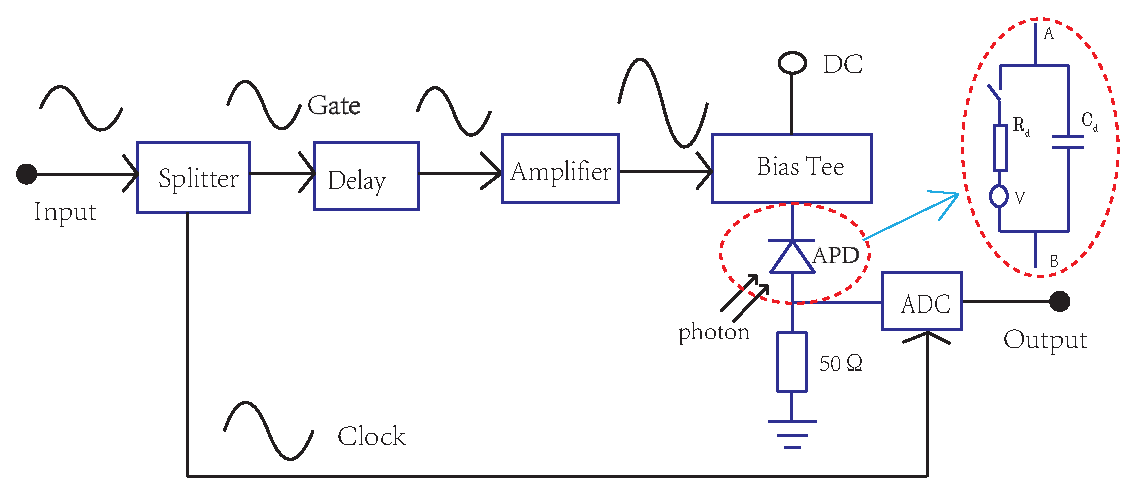
\includegraphics[width = 0.45\textwidth]{scheme.eps}% Here is how to import EPS art
\vskip -0.1in
\caption{\label{fig:diagram} Diagram of DS-SPAD. The sinusoidal signal is split into two portion, one is used as the gate of the APD and the other is used as the ADC sampling clock. The photon is fiber coupled to the APD.}
\vskip -0.2in
\end{figure}

In this work, we present a high digital sampling single photon avalanche detector (DS-SPAD), which can work at tunable gate repetition frequency using an ADC circuit at room temperature. Instead of restricting the spike noise by self-differencing or filtering, we %use sinusoidal wave as the gate instead of pulse gate in \cite{Seigo-adc2007} and
use an ADC to sampling the output voltage of the APD. %, a superimposing of spike noise and avalanche signal.
This detector implements continuous tunable gate repetition frequency which is under test from 900MHz to 1100MHZ while theoretically it can be worked at a wider range of repetition frequency.

\begin{figure}
\centering
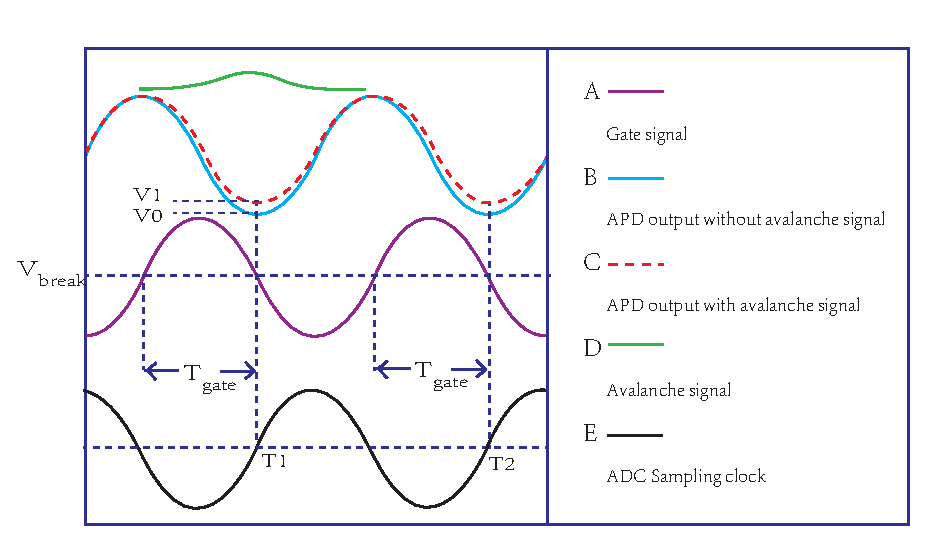
\includegraphics[width = 0.45\textwidth]{adc1.eps}
\vskip -0.1in
\caption{\label{fig:timing} Time relation between the APD gate signal, ADC sampling clock and the output signal. $V_{break}$ is the breakdown voltage of the APD. T1 and T2 are the sampling time of the ADC. $T_{gate}$ is the gate width.}
\vskip -0.2in
\end{figure}

The diagram of our DS-SPAD is shown in \autoref{fig:diagram}. In the diagram, an external sinusoidal clock is power split into two sinusoidal waves, i.e. $Gate$ and $Clock$. $Gate$ is used as the gate of the APD and $Clock$ is used as the sampling clock of the ADC. %In this way, the APD gate and the ADC sampling clock are at exactly the same frequency and are synchronized.
The ${Delay}$ is used to adjust the time difference between the $Clock$ and the $Gate$. Then the $Gate$ will be amplified by a tunable amplifier. Following the amplifier, the appropriate amplified $gate$ will be coupled with a DC voltage by a bias tee module. Finally the output of the APD is connected to the input of the ADC. A digitalized value will be outputted by the ADCs at every period clock.

%At 1GHz gate frequency we obtain a dark count rate of $3\times10^{-5}$ and 0.4\% afterpulse probability with 1 gate dead time at 10\% detection efficiency.  These features make the device suitable for a wide range of applications requiring high count rate, low noise, and fast NIR single photon detection. Moreover, the tunable gate frequency makes the device adaptable to meet the changing frequency applications.
%Although Negative feedback avalanche photodiode (NFAD) can work on free running mode, it needs a long deadtime, nearly 22\textmu s, which limits the count rate\cite{Ryan-NFAD2009,Korzh-NFAD2014}.

The APD is simply equivalent to the circuit shown as the inset of \autoref{fig:diagram}\cite{SCova-photodiodes1996}. %The diode is equivalent to a capacitance $C_d$.
With the charge and discharge effect of the $C_d$, when a sinusoidal signal shown as $A$ in \autoref{fig:timing} is input onto the APD, a response noise shown as $B$ will be generated on it. In this case, when a photon comes in the gate and triggers an avalanche, the output signal of the APD will be a superimpose of the response noise and the weak avalanche signal, shown as $C$. Here the avalanche signal shown as $D$ is much weaker than the response noise. The output voltage of the APD with avalanche signal superimposed will be slightly higher than the voltage without avalanche signal, shown as ${V1}$ and ${V0}$ at time ${T1}$. %In this way, if we obtain the value of the output signal at time ${T1}$, then we can tell whether there is an avalanche occurs or not. From the above analysis, we can know that
Since the frequency of the ADC sampling clock and the APD gate are exactly the same and synchronized, then by adjusting the $delay$ we can sample the signal exactly at point ${T1}$ in every period and obtain one sampling value of the output signal at every gate. By comparing the sampling value we can judge whether there is an avalanche occurs or not. Since there is no frequency strongly dependent devices, the sinusoidal gate frequency can be quite broad theoretically instead of a fix frequency, which makes the gate repetition frequency of the detector tunable.
\begin{figure}
%begin{tabular}{cc}
\begin{minipage}{0.45\linewidth}
\centering
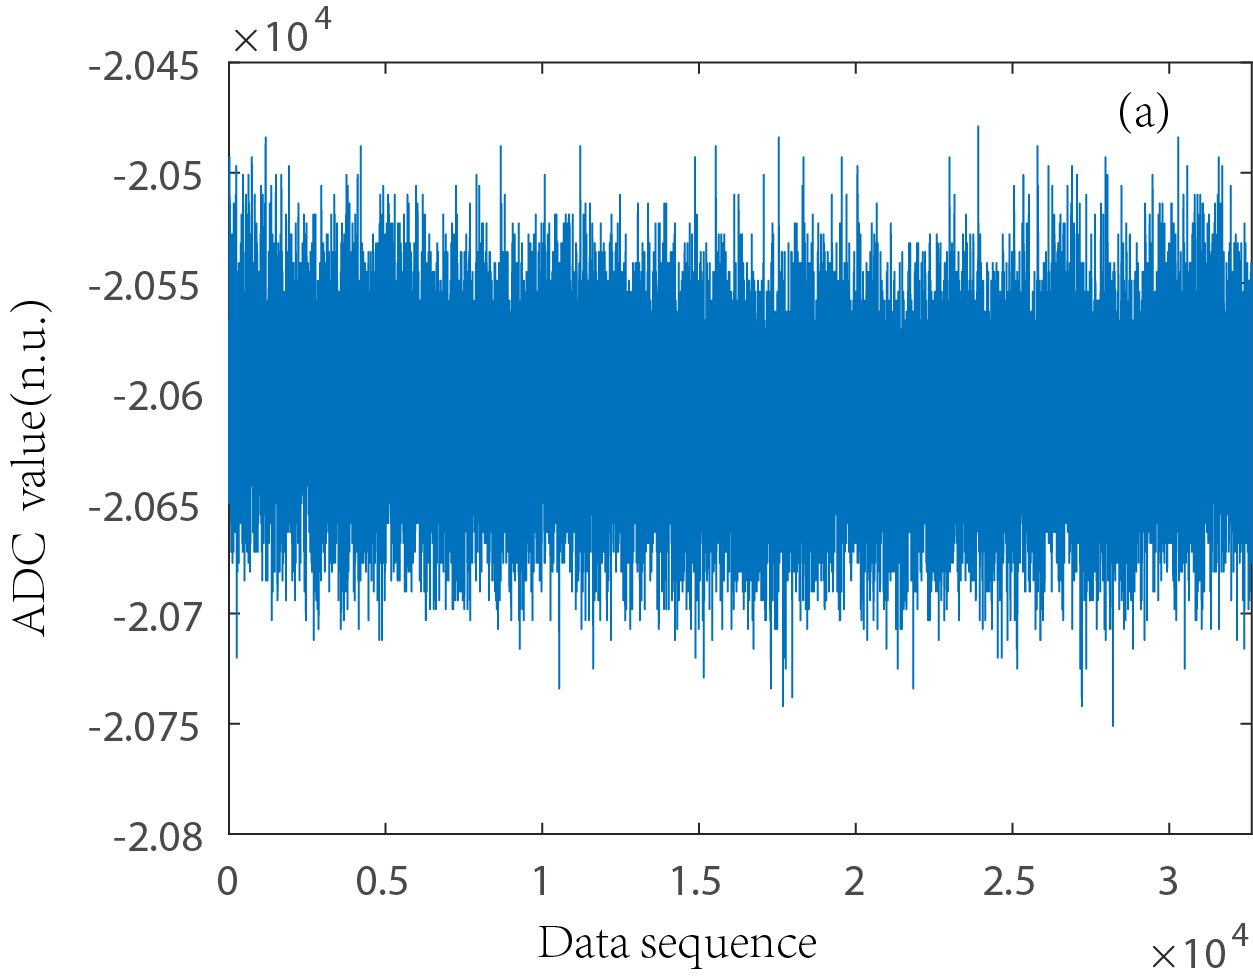
\includegraphics[width = 1\textwidth]{figure/no-counts-biased.jpg}% no-counts-100M-1.2V-66.1V-6-biased
\end{minipage}
\begin{minipage}{0.45\linewidth}
\centering
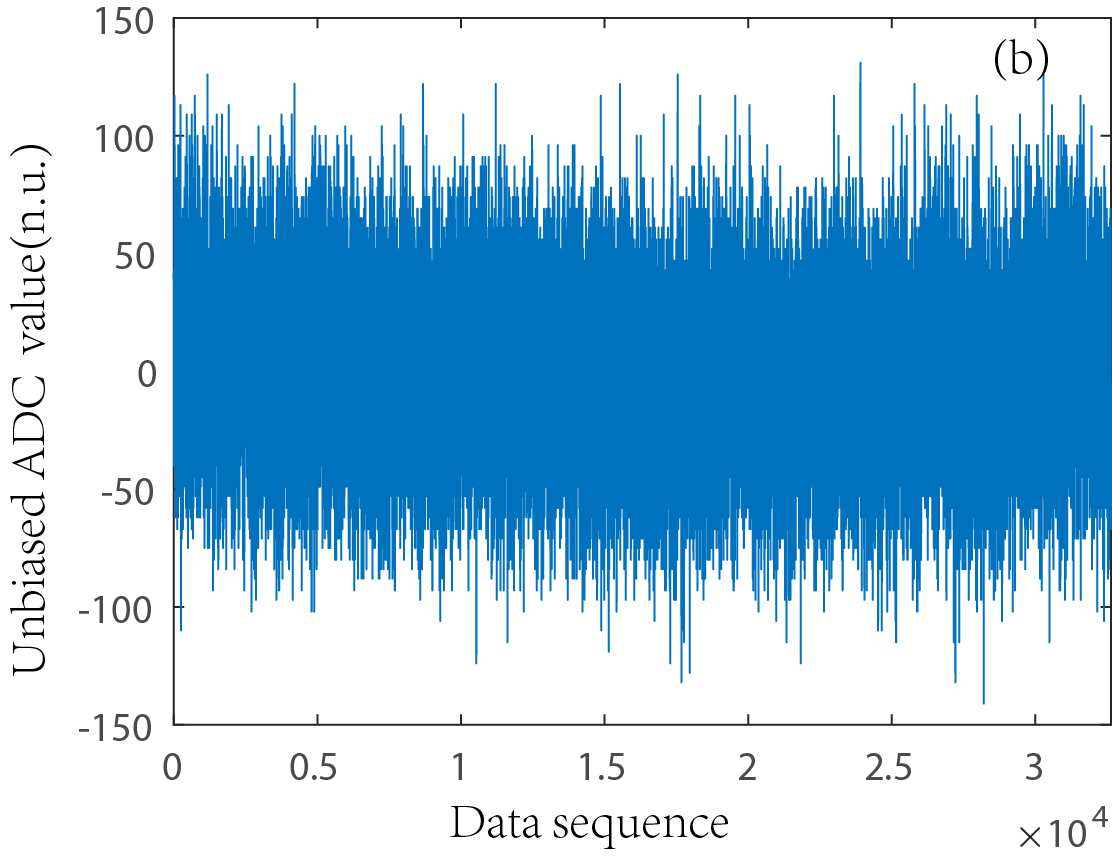
\includegraphics[width = 1\textwidth]{figure/no-counts.jpg}% Here is how to import EPS art
\end{minipage}

\begin{minipage}{0.45\linewidth}
\centering
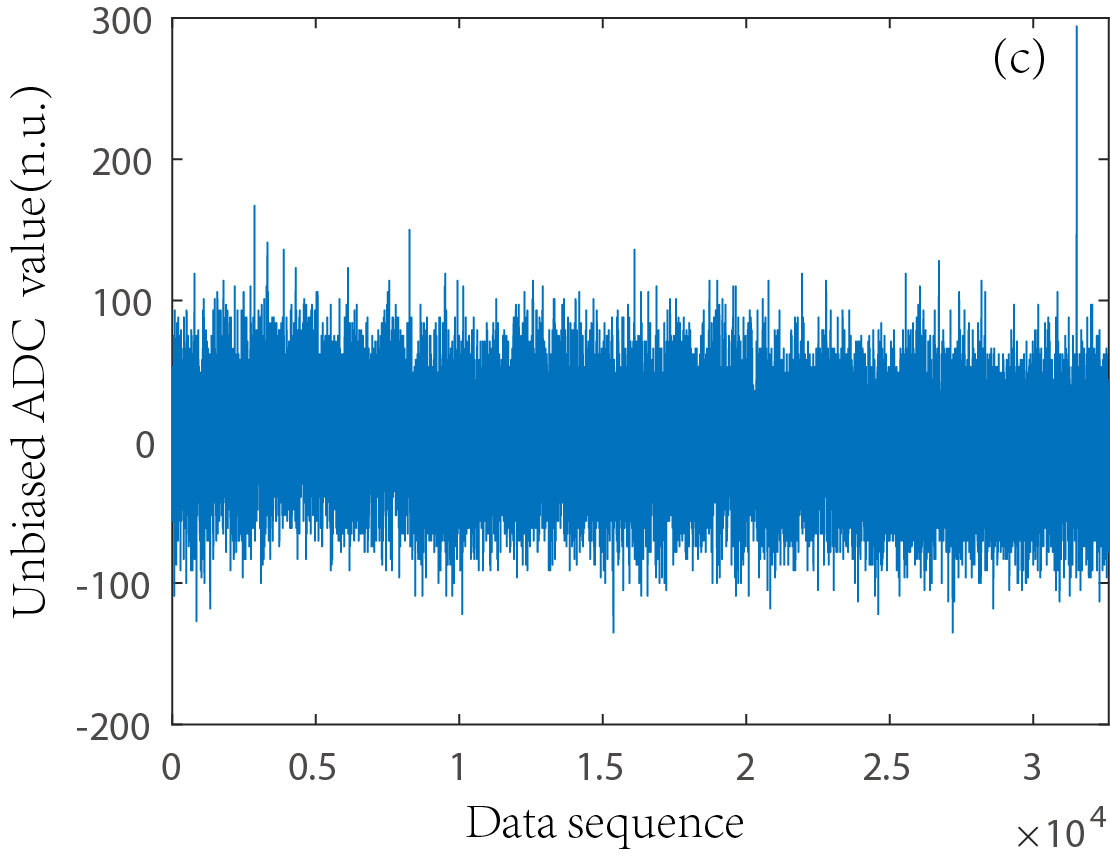
\includegraphics[width = 1\textwidth]{figure/1-count.jpg}%
\end{minipage}
\begin{minipage}{0.45\linewidth}
\centering
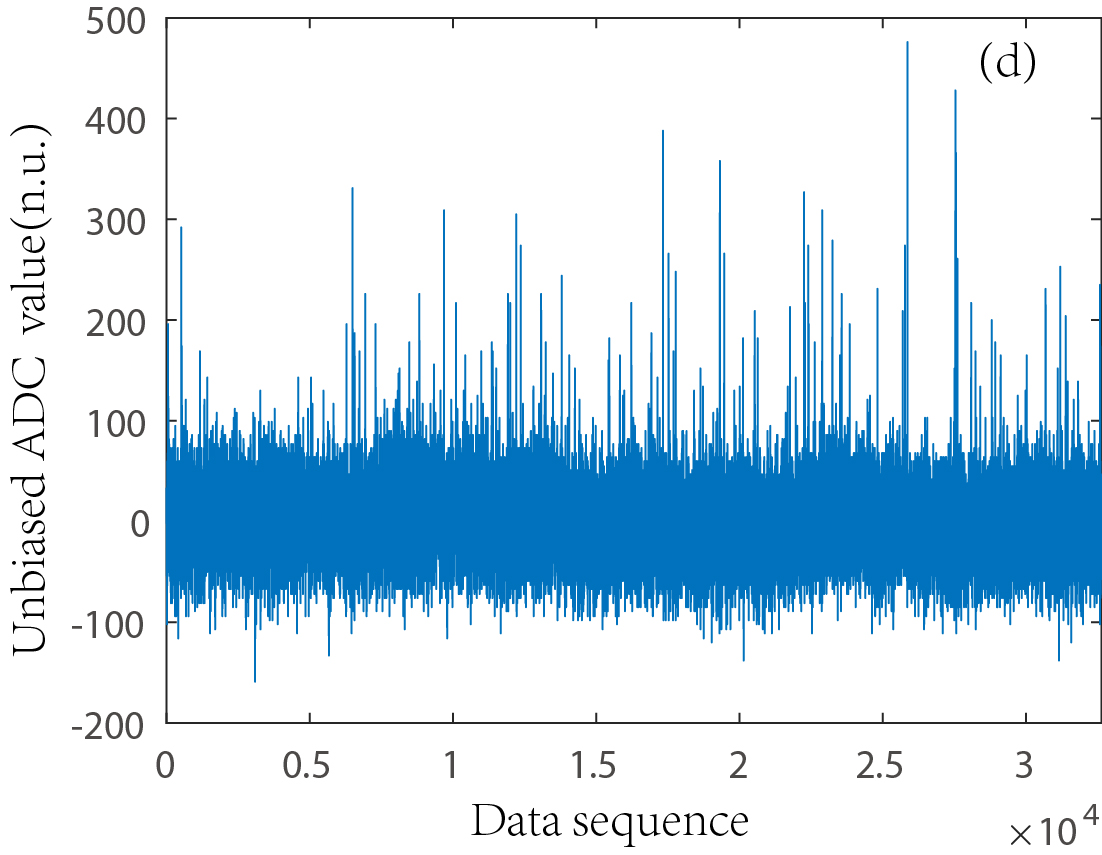
\includegraphics[width = 1\textwidth]{figure/10percent.jpg}%
\end{minipage}
\vskip -0.1in
\caption{\label{fig:ADC_output}(a) the direct digital output of ADC with no avalanche signal, (b)unbiased output of (a), (c)unbiased output with one dark count avalanche signal, (d)unbiased output with 0.1 photon per pulse on average incident. One data represents one gate and the gate frequency is 1GHz.}
\vskip -0.2in
\end{figure}
%In our experiment, we use an external clock which is synchronized with the gate to trigger to sample the APD output signal.


\begin{figure}
\centering
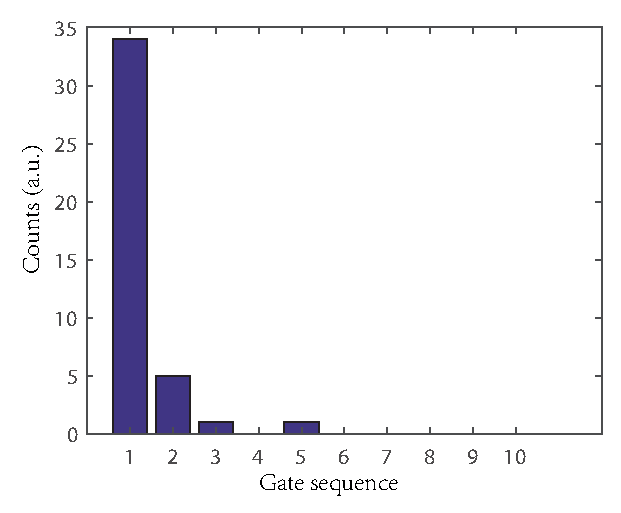
\includegraphics[width = 0.3\textwidth]{figure/bar-10percent.eps}% Here is how to import EPS art
\vskip -0.1in
\caption{\label{fig:counts_bar} The accumulation of detected counts of \autoref{fig:ADC_output}(d) at every 10th gate. For example, the first bar shows the accumulation count of gate 1, gate 11, gate 21, and so forth.}
\vskip -0.2in
\end{figure}

\begin{figure*}
%begin{tabular}{cc}
\begin{minipage}{0.24\linewidth}
\centering
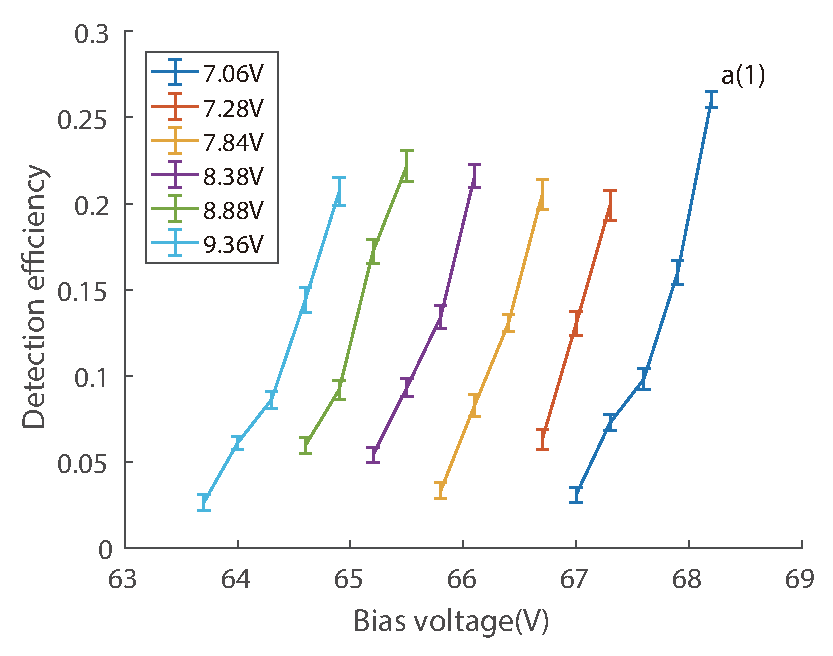
\includegraphics[width = 1\textwidth]{figure/90M/efficiency.eps}% no-counts-100M-1.2V-66.1V-6-biased
\end{minipage}
\begin{minipage}{0.24\linewidth}
\centering
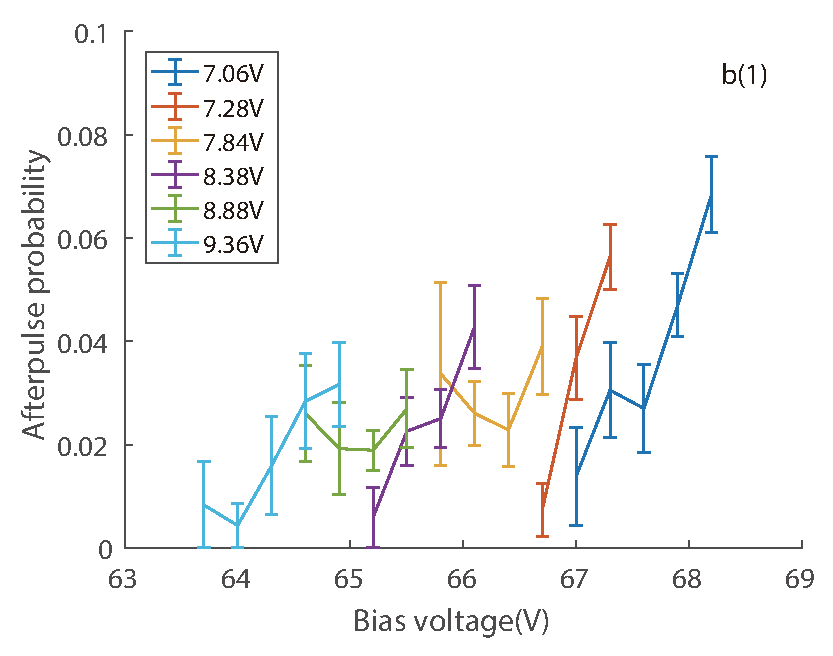
\includegraphics[width = 1\textwidth]{figure/90M/afterpulse0.eps}% no-counts-100M-1.2V-66.1V-6-biased
\end{minipage}
\begin{minipage}{0.24\linewidth}
\centering
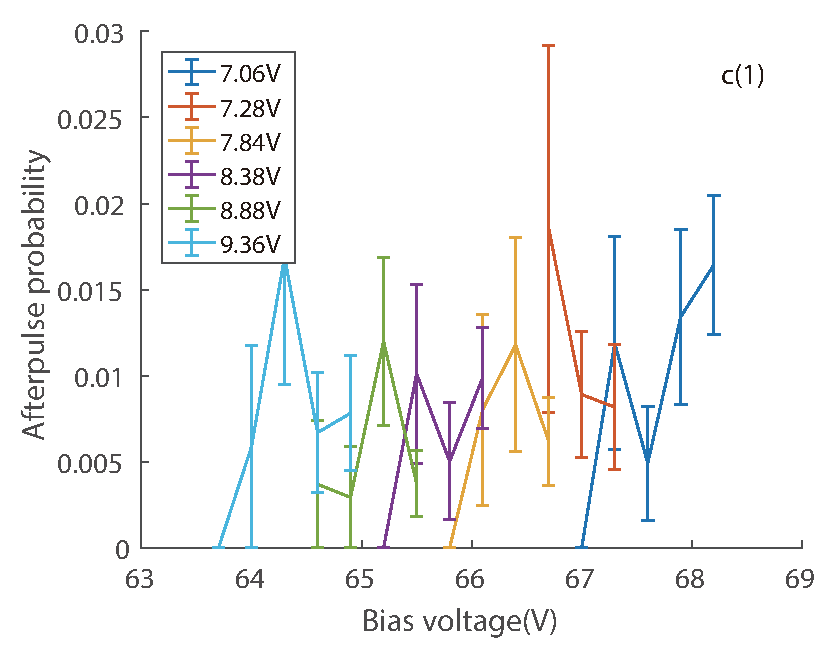
\includegraphics[width = 1\textwidth]{figure/90M/afterpulse1.eps}% no-counts-100M-1.2V-66.1V-6-biased
\end{minipage}
\begin{minipage}{0.24\linewidth}
\centering
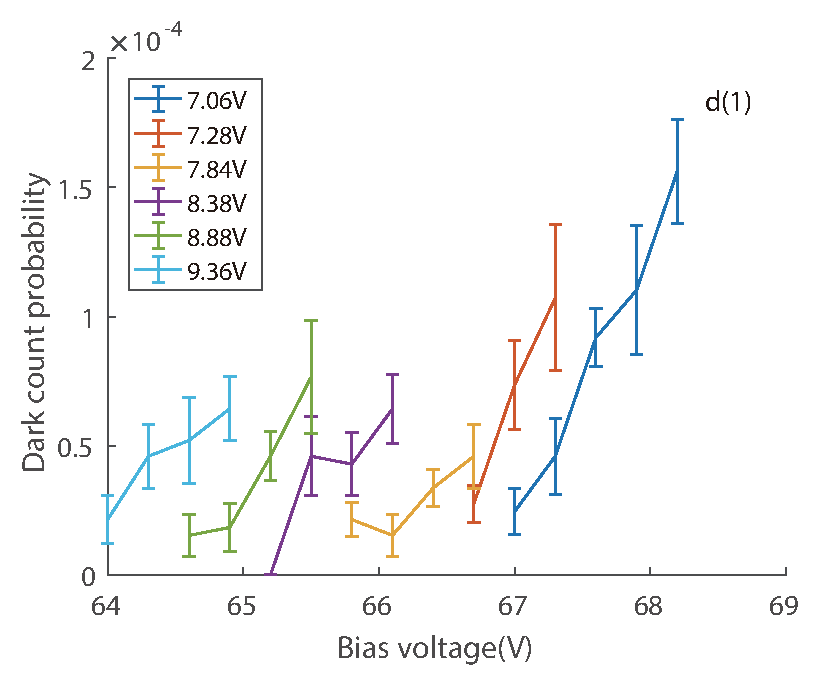
\includegraphics[width = 1\textwidth]{figure/90M/darkcount.eps}% no-counts-100M-1.2V-66.1V-6-biased
\end{minipage}

\begin{minipage}{0.24\linewidth}
\centering
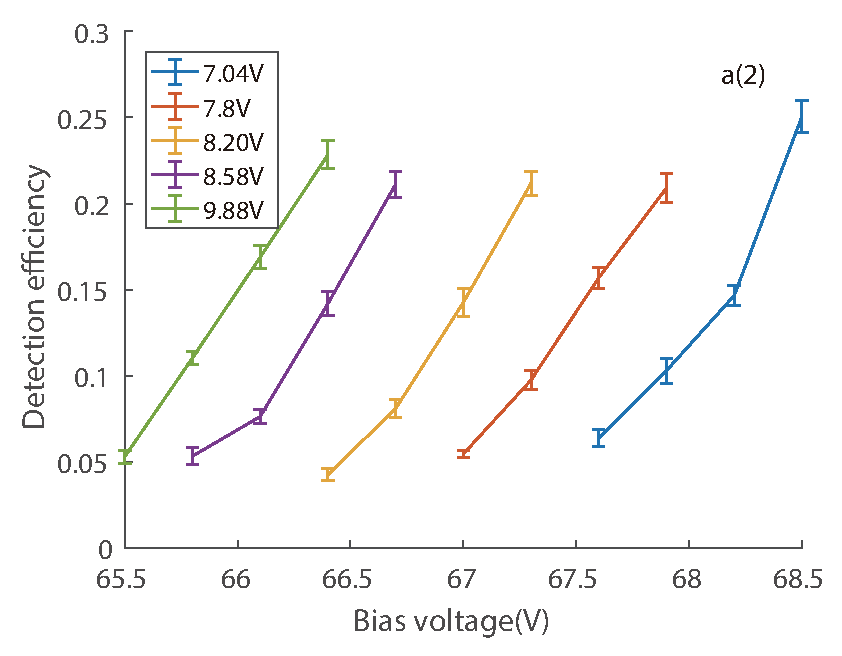
\includegraphics[width = 1\textwidth]{figure/95M/efficiency.eps}% no-counts-100M-1.2V-66.1V-6-biased
\end{minipage}
\begin{minipage}{0.24\linewidth}
\centering
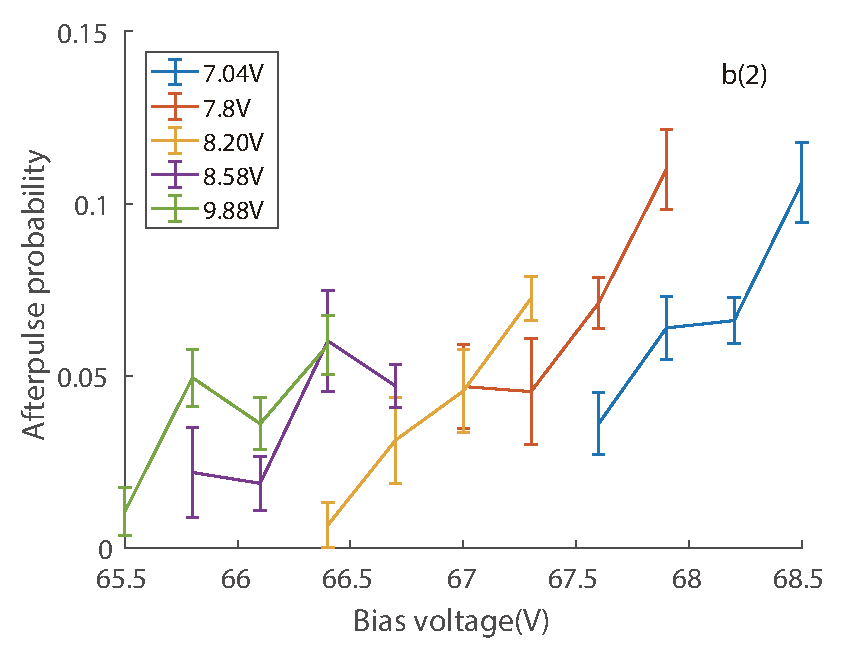
\includegraphics[width = 1\textwidth]{figure/95M/afterpulse0.eps}% no-counts-100M-1.2V-66.1V-6-biased
\end{minipage}
\begin{minipage}{0.24\linewidth}
\centering
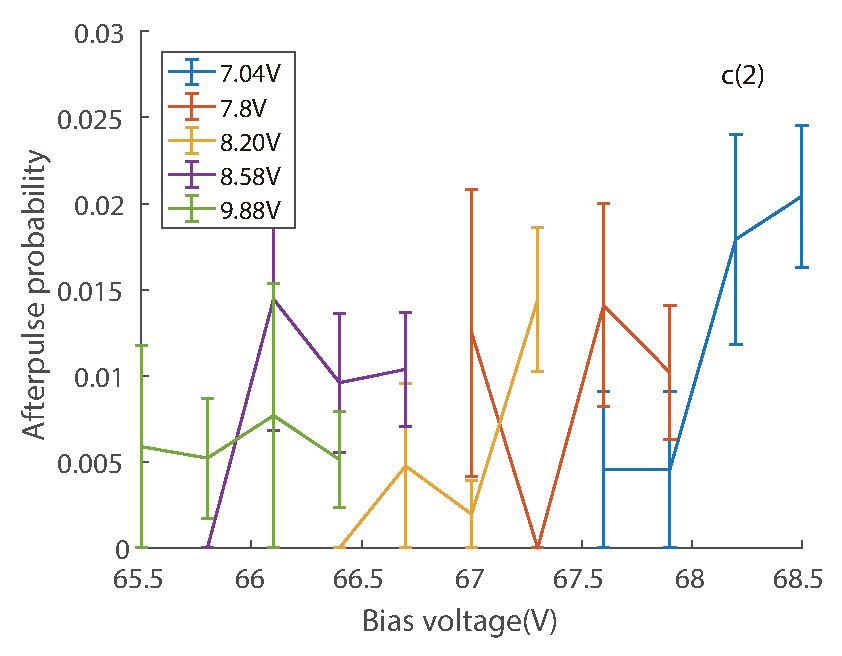
\includegraphics[width = 1\textwidth]{figure/95M/afterpulse1.eps}% no-counts-100M-1.2V-66.1V-6-biased
\end{minipage}
\begin{minipage}{0.24\linewidth}
\centering
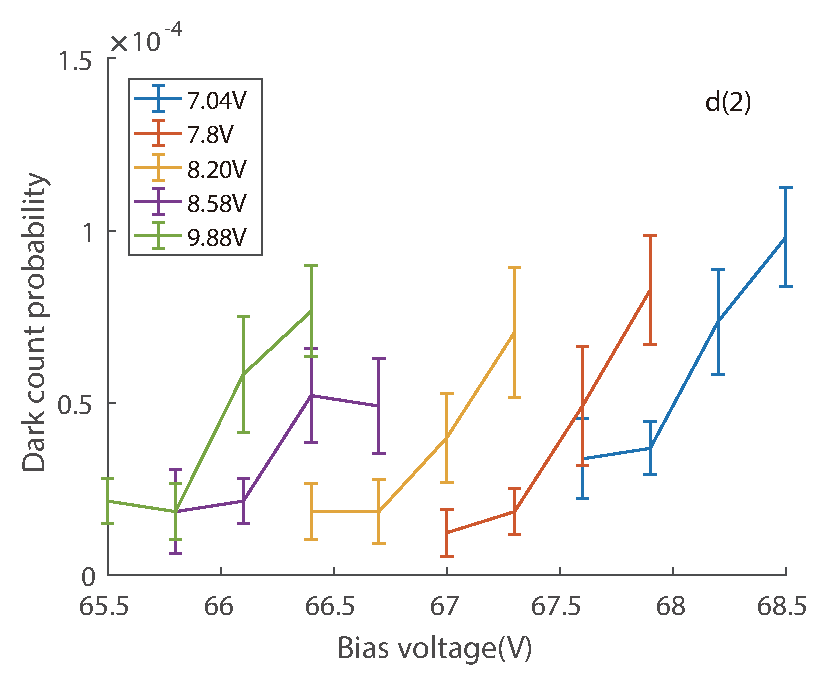
\includegraphics[width = 1\textwidth]{figure/95M/darkcount.eps}% no-counts-100M-1.2V-66.1V-6-biased
\end{minipage}

\begin{minipage}{0.24\linewidth}
\centering
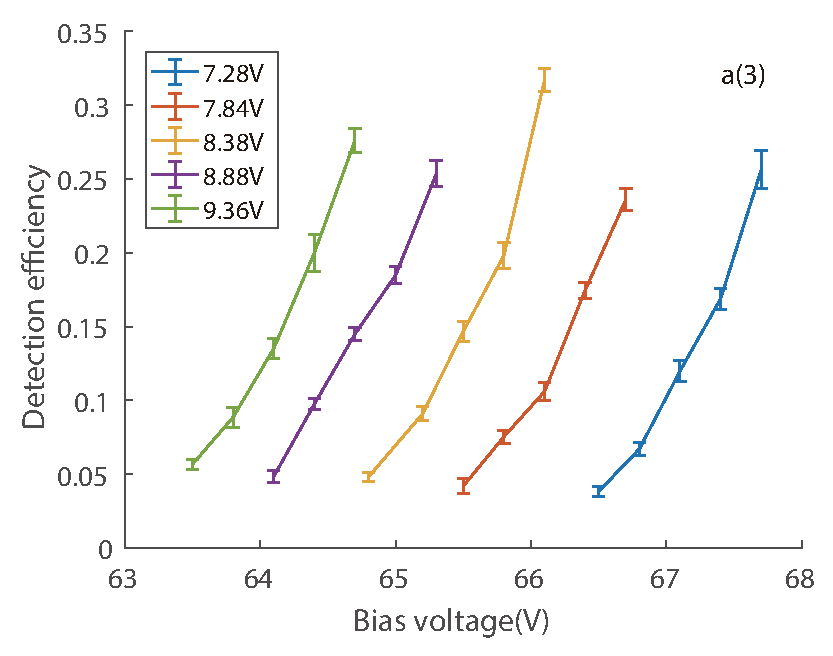
\includegraphics[width = 1\textwidth]{figure/100M/efficiency.eps}% no-counts-100M-1.2V-66.1V-6-biased
\end{minipage}
\begin{minipage}{0.24\linewidth}
\centering
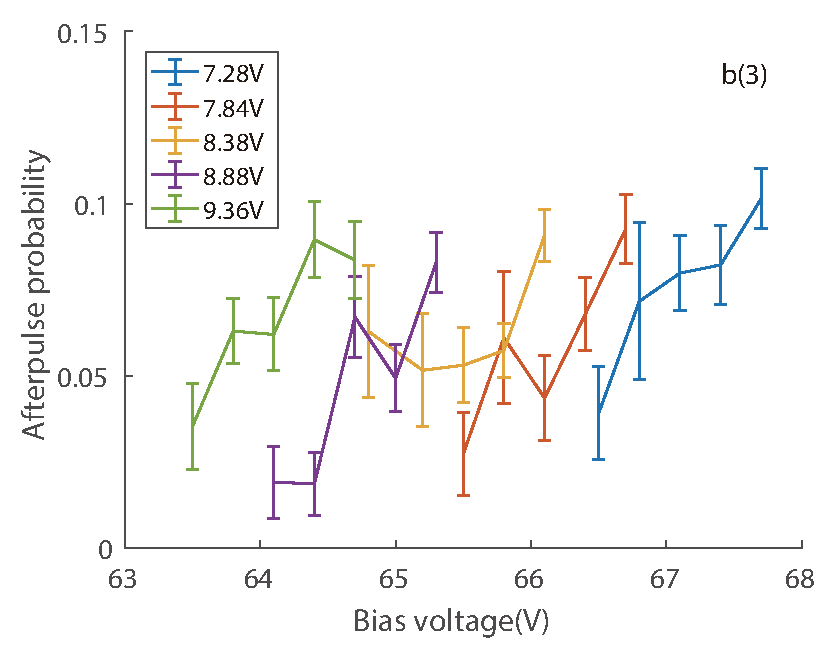
\includegraphics[width = 1\textwidth]{figure/100M/afterpulse0.eps}% no-counts-100M-1.2V-66.1V-6-biased
\end{minipage}
\begin{minipage}{0.24\linewidth}
\centering
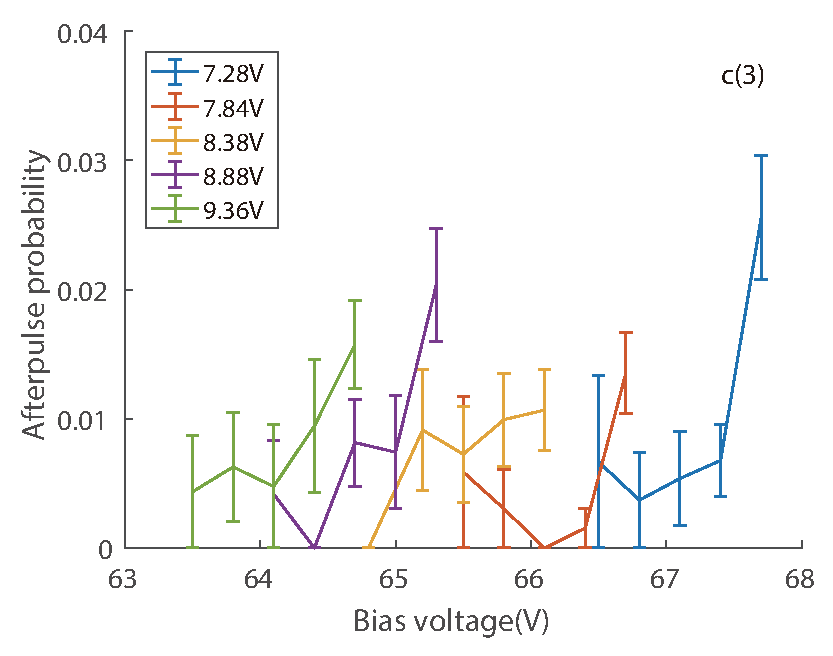
\includegraphics[width = 1\textwidth]{figure/100M/afterpulse1.eps}% no-counts-100M-1.2V-66.1V-6-biased
\end{minipage}
\begin{minipage}{0.24\linewidth}
\centering
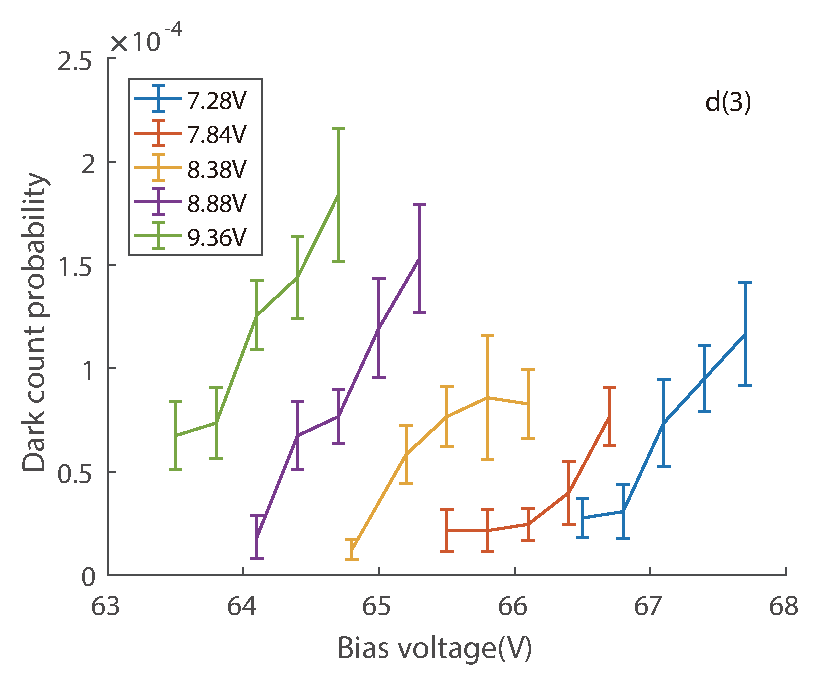
\includegraphics[width = 1\textwidth]{figure/100M/darkcount.eps}% no-counts-100M-1.2V-66.1V-6-biased
\end{minipage}

\begin{minipage}{0.24\linewidth}
\centering
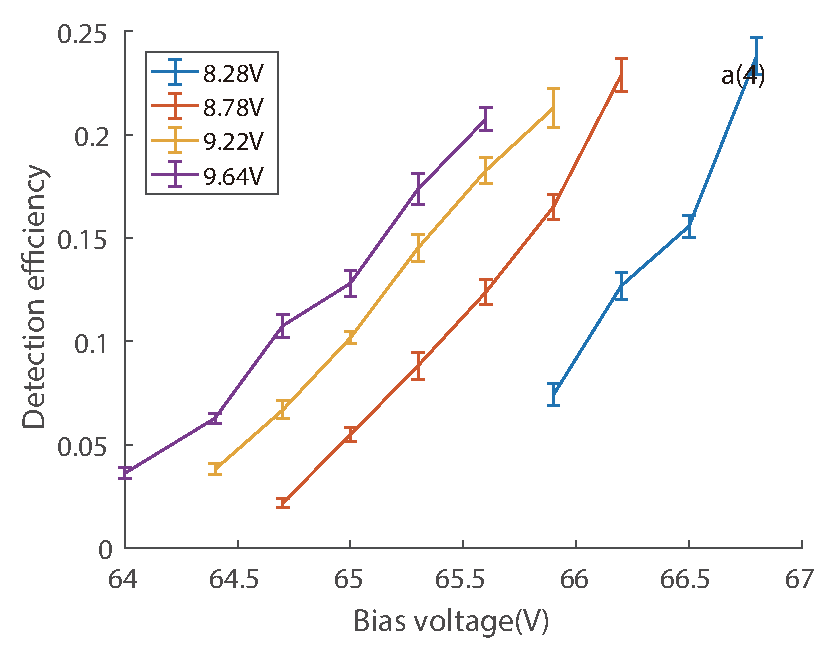
\includegraphics[width = 1\textwidth]{figure/105M/efficiency.eps}% no-counts-100M-1.2V-66.1V-6-biased
\end{minipage}
\begin{minipage}{0.24\linewidth}
\centering
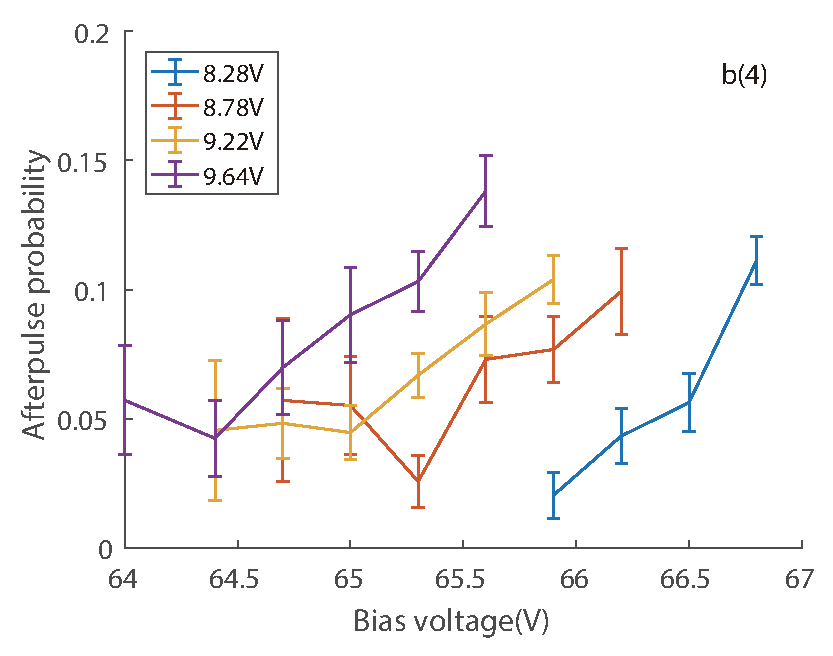
\includegraphics[width = 1\textwidth]{figure/105M/afterpulse0.eps}% no-counts-100M-1.2V-66.1V-6-biased
\end{minipage}
\begin{minipage}{0.24\linewidth}
\centering
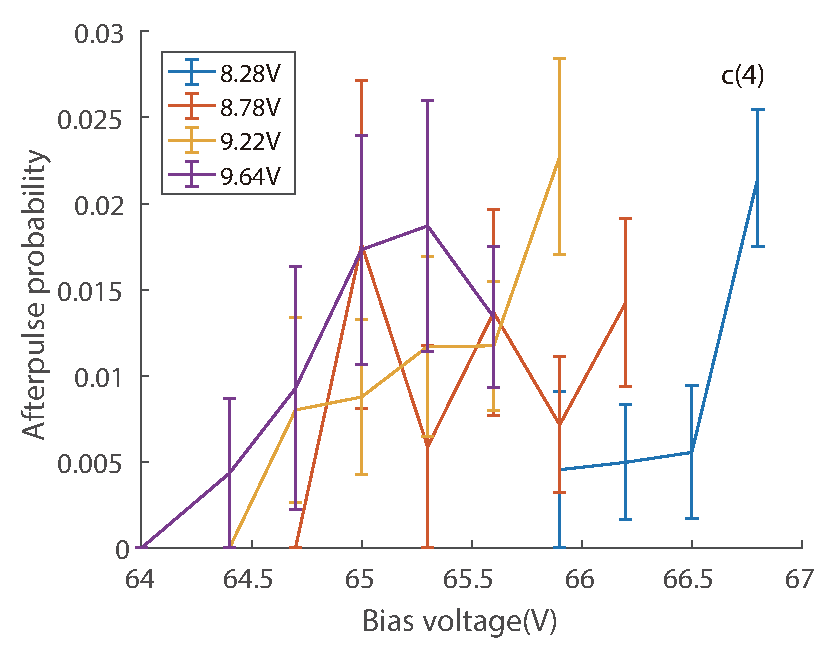
\includegraphics[width = 1\textwidth]{figure/105M/afterpulse1.eps}% no-counts-100M-1.2V-66.1V-6-biased
\end{minipage}
\begin{minipage}{0.24\linewidth}
\centering
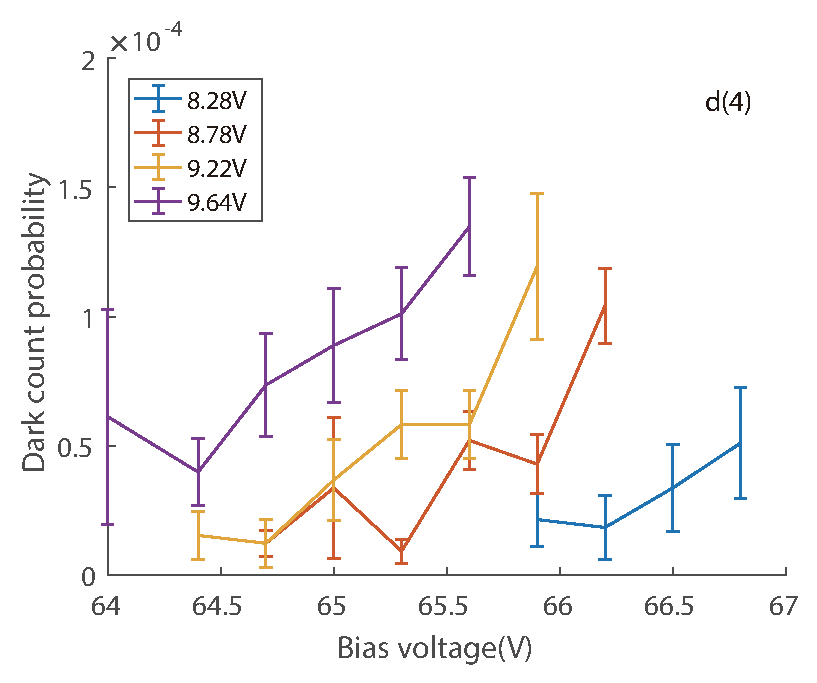
\includegraphics[width = 1\textwidth]{figure/105M/darkcount.eps}% no-counts-100M-1.2V-66.1V-6-biased
\end{minipage}

\begin{minipage}{0.24\linewidth}
\centering
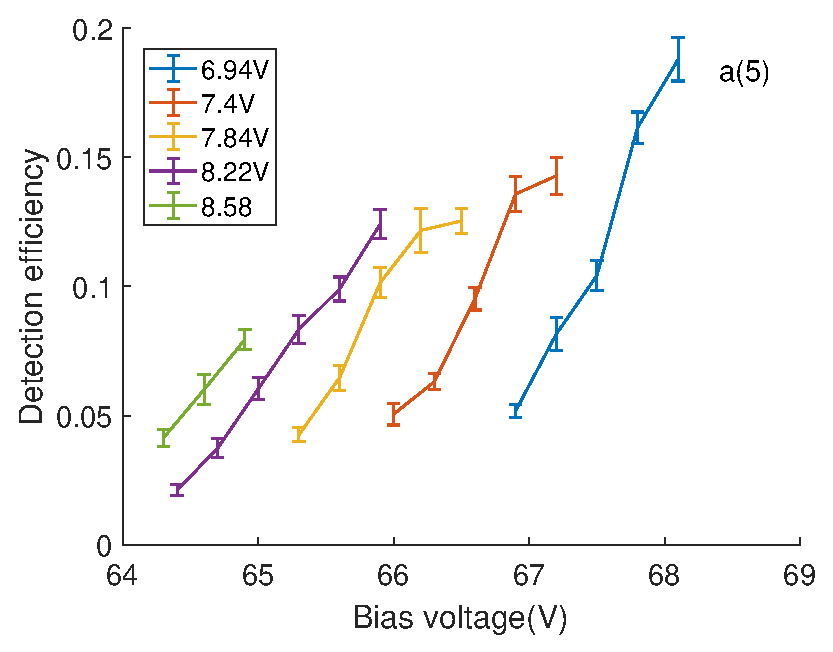
\includegraphics[width = 1\textwidth]{figure/110M/efficiency.eps}% no-counts-100M-1.2V-66.1V-6-biased
\end{minipage}
\begin{minipage}{0.24\linewidth}
\centering
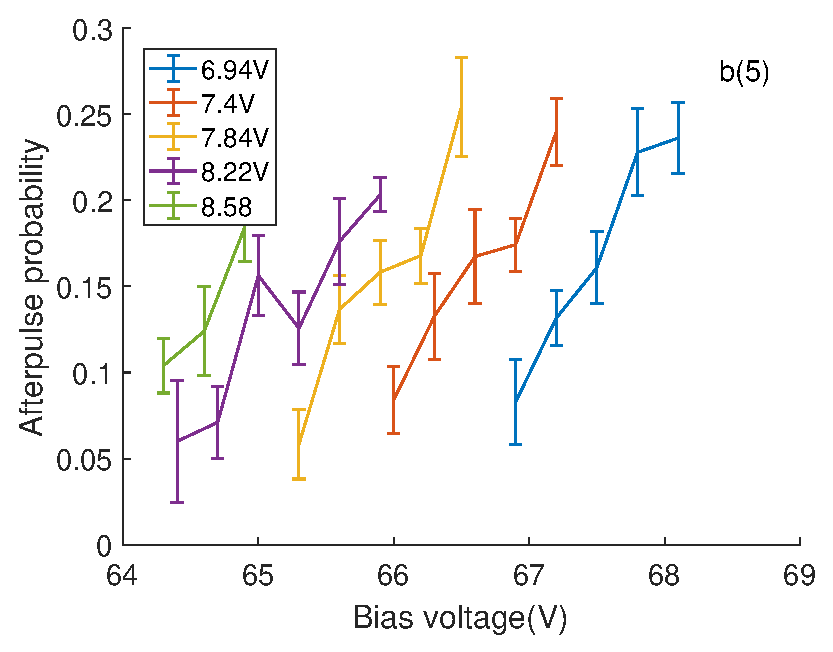
\includegraphics[width = 1\textwidth]{figure/110M/afterpulse0.eps}% no-counts-100M-1.2V-66.1V-6-biased
\end{minipage}
\begin{minipage}{0.24\linewidth}
\centering
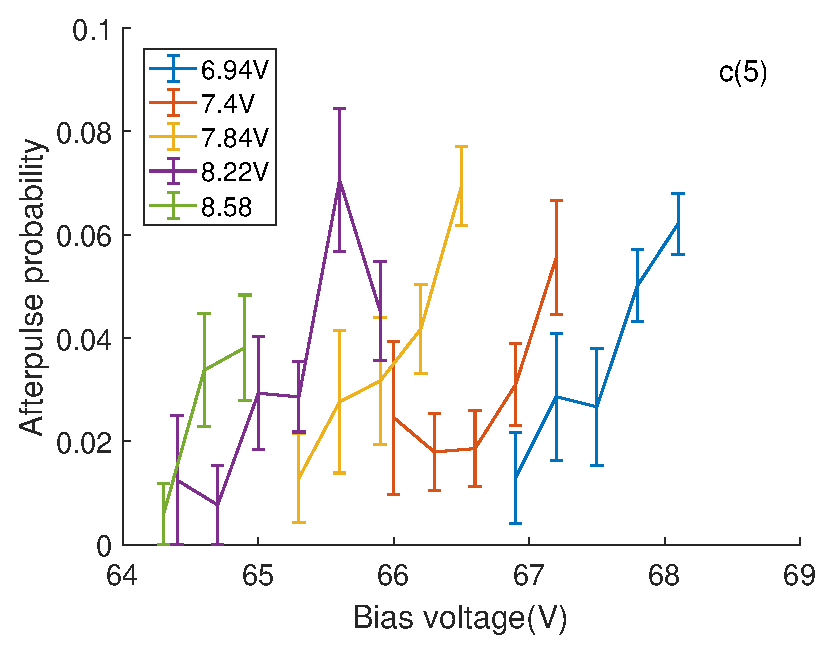
\includegraphics[width = 1\textwidth]{figure/110M/afterpulse1.eps}% no-counts-100M-1.2V-66.1V-6-biased
\end{minipage}
\begin{minipage}{0.24\linewidth}
\centering
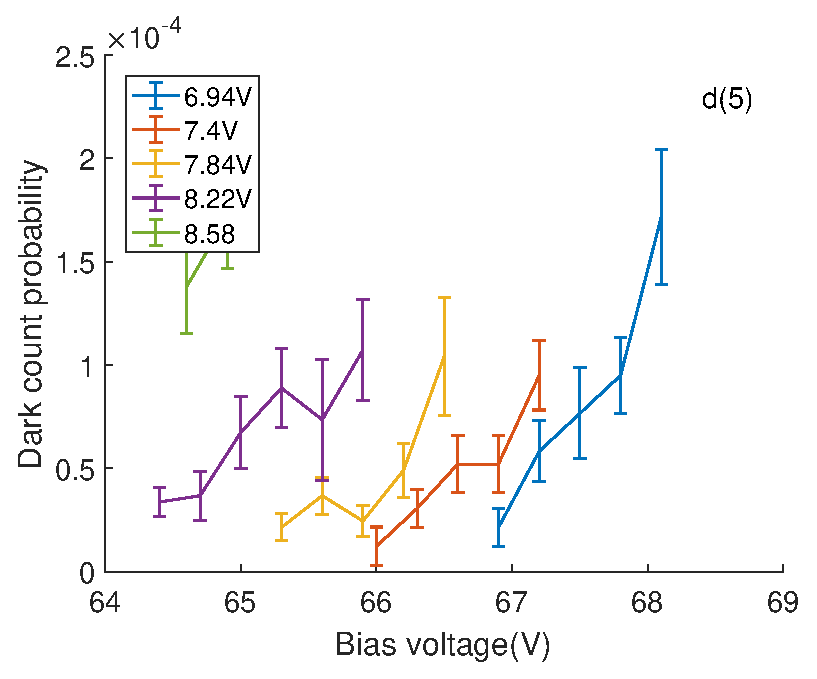
\includegraphics[width = 1\textwidth]{figure/110M/darkcount.eps}% no-counts-100M-1.2V-66.1V-6-biased
\end{minipage}
\vskip -0.1in
\caption{\label{fig:specifics}The figures in the first row are measured at 900MHz gate repetition frequency and the second row at 950MHz, the third at 1000MHz, the fourth row at 1050MHz and fifth row at 1100MHz. The first column a(1)-a(5) show the detection efficiencies. The second column b(1)-b(5) show the afterpulse probabilities with no additional deadtime. The third column c(1)-(c5) show the afterpulse probabilities with 1 gate additional deadtime. The fourth column d(1)-d(5) show the dark count probabilities. The legend values in each figure are the peak-peak voltage of the sinusoidal gate, and the horizontal axis values are the bias voltage added to the sinusoidal gate.}
\vskip -0.2in
\end{figure*}

% There is a point needs to be mentioned that in our scheme we need to adjust the amplitude and the DC bias to set the breakdown voltage more or less at the center or the sine gate to ensure the timing showed in \autoref{fig:timing} or else the avalanche signal will be shifted.

The ADC used here is ADQ7 with 14bits resolution. It will sample a value when a rise edge of the sampling clock occurs and then digitalize it. The ENOB (Equivalent Number of Bits) of the device at 2.5GHz clock is 7.3, $2^{7.3} \approx $158, that means the resolution ratio is about 0.6\%. %To analyze the detection efficiency, dark count probability and afterpulse probability,
In the experiment, the ADC outputs are saved into 16bits of binary format files for processing. %In this way, it is easier to process the data with Matlab or other tools.
The ADC also provides a real time processing module FPGA, which is essential for practical use. The InGaAs APD used in our experiment is commercially available from Princeton Lightwave. The beakdown voltage is -71V at 25$^{\circ}$C. In the experiment, the InGaAs APD worked at room temperature of 21$^{\circ}$C. We use a homemade pulsed laser diode at 1.55\textmu m with a pulse duration of 50$ps$ to act as single photon source. The laser is attenuated to 0.1 photon per pulse on average by the optical attenuator before coupling into the APD fiber pigtail. In addition, the laser pulse is 1/10th synchronized to the gate frequency which means if the gate frequency is 1GHz, then the laser pulse frequency is 100MHz. \autoref{fig:ADC_output} (a) is the direct digital output of ADC with laser switched off and no dark count occurs. The vertical axis value of \autoref{fig:ADC_output} (a) is the digital converted value of the sampling data. For instance, the value $-2.06\times10^4$ represents that the sampling point voltage value is $\frac{FS}{2} \times(-2.06\times10^4)/2^{15}$, where FS is the Full-scale voltage of the ADC and is 1V for ADQ7. So the average voltage of the response noise at the sampling point shown in \autoref{fig:ADC_output} (a) is -315.9mV and the fluctuation of the response noise at the sampling point is $1V \times 200/2^{16} \approx 3.1mV$. When applying different gate amplitude, the average voltage of the response noise would be different. It would be inconvenient to set the threshold value. Here we subtract the mean value of \autoref{fig:ADC_output} (a) and only get the fluctuation value shown in \autoref{fig:ADC_output} (b). \autoref{fig:ADC_output} (c) is a processed output with laser switched off and one dark count occurs. \autoref{fig:ADC_output} (d) is a processed output with laser switched on. We can clearly see the avalanche signal the highest avalanche signal voltage is about $1V \times 500/2^{16} \approx 7.6mV$. For each measurement, the ADC samples 32634 data. %So the discrimination threshold can be set as 250.
As only 1/10th of the gate is with photon input, we can plot the detected counts respected to gates sequence into \autoref{fig:counts_bar}. The vertical axis is the accumulated counts of detected photons. The horizontal axis 'Gate sequence' means that Gate sequence 1 is the accumulation of gate 1, gate 11 of ADC gate and so on, Gate sequence 2 is the accumulation of gate 2, gate 12 of ADC and so on, and the same for Gate sequence 3 to Gate sequence 10. Gate sequence 1 are the gates with photon incident, while others are with no photon incident. Here we define $R_{i}$ to be the accumulation count at $i$th Gate sequence.

\begin{table*}
\vskip -0.1in
\caption{\label{tab:comparison}
A comparison of our results with the other reported high-speed SPDs. $P_e$ is the detection efficiency, $P_a$ is the afterpulse probability, $P_d$ is the dark count probability.}
\begin{ruledtabular}
\begin{tabular}{cccccccc}
&temperature &frequency &$P_e$ &$P_a$ &$P_d$ &deadtime &working mode\\ \hline
sinusoidal gate\cite{Pan-sine2012}& -50 $^{\circ}$C & 1.25GHz & 10\% & 11.7\% &$4.66\times10^{-6}$
& 0\footnote{0 dead time represents dead time free}  & fixed gating \\
sinusoidal gate\cite{NKata-sine2009}& -60 $^{\circ}$C & 1.5GHz & 10.8\% & 2.8\% &$6.3\times10^{-7}$
& 50\textmu s & fixed gating  \\
self-differencing\cite{Zhang-practical2009}& -30 $^{\circ}$C & 921MHz & 9.3\% & 3.4\% &$2.8\times10^{-6}$
& 10ns & fixed gating  \\
self-differencing\cite{Comandar-55efficeincy2015}& 20 $^{\circ}$C & 1GHz & 10\% & $\sim$ 2\% &$\sim 1.2\times10^{-5}$
& 0 & fixed gating  \\ \hline
\multirow{2}*{self-differencing\cite{Comandar2014Room-temperature}}& 20 $^{\circ}$C & 1GHz & 10\% & $\sim$ 1.7\% &$\sim 2\times10^{-5}$ & --\footnote{-- represents no data} & fixed gating  \\
& 20 $^{\circ}$C & 1GHz & 25\% & $\sim$ 2.8\% &$5.9\times10^{-5}$ & -- & fixed gating  \\ \hline
\multirow{2}*{self-differencing\cite{ZLYuan-Multi2010}}& -30 $^{\circ}$C &2GHz & 11.8\% & 1.43\% & $3.79\times10^{-6}$
& 0 & fixed gating \\
& -30 $^{\circ}$C &1GHz & 10\% & 2.5\% & $6.6\times10^{-6}$
& 0 & tunable gating(0.987 $\sim$ 1.033GHz ) \\ \hline
NFAD\cite{Korzh-NFAD2014}& -110 $^{\circ}$C & \-- & 10\% & 2.2\% &1Hz
& 20\textmu s & free running \\ \hline
\multirow{2}*{id210} & &\-- & 10\% & \-- &3.3KHz
& 50\textmu s & free running  \\
 & &\-- & 10\% & \-- &$2.04\times10^{-6}$
& 10\textmu s & fixed gating  \\ \hline
\multirow{2}*{ this work}& 21 $^{\circ}$C & 1GHz & 10\% & 0.4\% &$3\times10^{-5}$ & 1ns & tunable gating(0.9 $\sim$ 1.1GHz ) \\
& 21 $^{\circ}$C & 1GHz & 20\% & 0.7\% &$5.6\times10^{-5}$ & 1ns & tunable gating(0.9 $\sim$ 1.1GHz ) \\
\end{tabular}
\end{ruledtabular}
\end{table*}

We tested the detector at different gate repetition frequencies range from 900MHz to 1100MHz. The results are shown in \autoref{fig:specifics}. The values in the legends represent the gate peak-peak voltages. The dark count probability shown in \autoref{fig:specifics} d(1)-d(5) are measured by switching off the incident laser and counting the ADC outputs which exceed the threshold value. The dark count probability is defined as: $P_d = \frac{\sum_{i=1}^{10}R_{i} }{R_{gate}}$, where $R_{gate}$ is the total count of gate. The detection efficiency is calculated by: $P_e = 100\times R_{1}/R_{gate}$ and shown in \autoref{fig:specifics} a(1)-a(5). %They are measured by incidencing 0.1 photon per pulse on average at every 10th gate.
\autoref{fig:specifics} b(1)-b(5) show the first gate afterpulse probability which is defined as: $P_{a1} = R_{12}/R_1$, here $R_{12}$ is a conditional count that when there is a count in gate 1 and then also gets a count in the next gate, i.e. gate2.  Similarly, \autoref{fig:specifics} c(1)-c(5) show the second gate afterpulse probability which is defined as: $P_{a1} = R_{13}/R_1$, where $R_{13}$ is a conditional count that when there is a count in gate 1 and then also gets a count in gate3. The afterpulse of third and other gates are not shown here, because they are decreased to below 0.1\%. Combine \autoref{fig:specifics} a(1)-a(5) and  \autoref{fig:specifics} d(1)-d(5), we can see that for each gate repetition frequency, there is an optimum peak-peak voltage to achieve optimum dark count probability. The optimum peak-peak voltages are 7.84V, 7.8V, 7.84v, 8.28V and 7.84V at 900MHz, 950MHz, 1000MHz, 1050MHz and 1100MHz gate repetition frequency respectively. The optimum peak-peak voltages show a very nice consistency. To get a more clear comparison of the performance at different repetition frequency, we select the datasets of detection efficiency, afterpulse probability and dark count probability  measured at  7.84V, 7.8V, 7.84v, 8.28V and 7.84V peak-peak voltage at 900MHz 950MHz, 1000MHz, 1050MHz and 1100MHz respectively. Then we do the linear fit to the data. \autoref{fig:fit} shows the mean value with error bars and fitting lines of the detection efficiency, dark count probability and afterpulse probability with 0, 1 and 2 gates of dead time. From the fitted line, we obtain the afterpulse probability and dark count probability at 10\%, 15\% and 20\% detection efficiency, which are shown in \autoref{fig:afterpulse_darkcount_rate}.

\begin{figure}
%begin{tabular}{cc}
\begin{minipage}{0.45\linewidth}
\centering
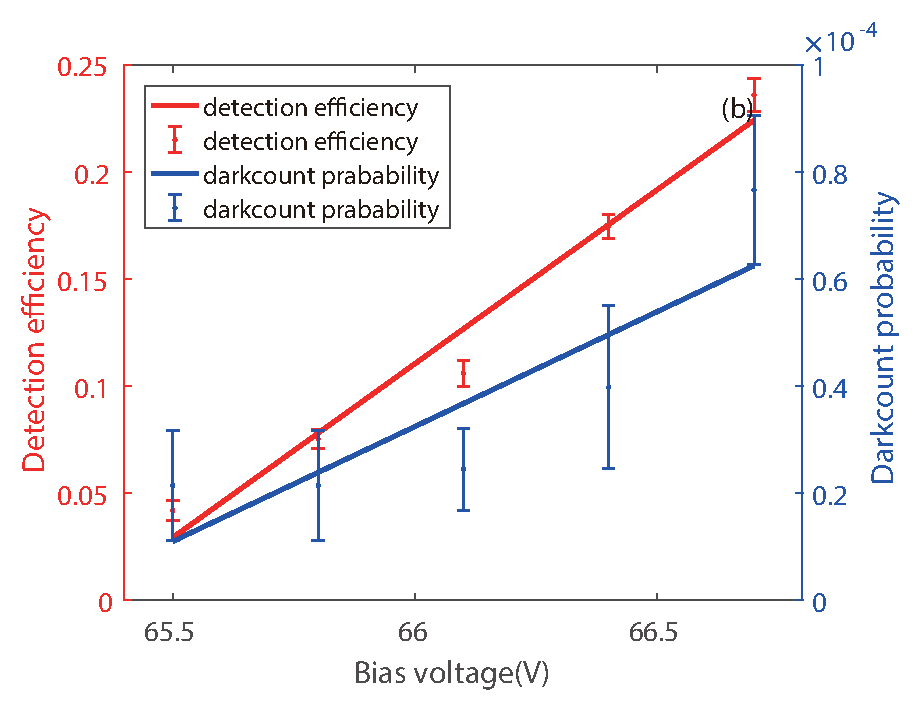
\includegraphics[width = 1\textwidth]{figure/darkcount_fit.eps}% no-counts-100M-1.2V-66.1V-6-biased
\end{minipage}
\begin{minipage}{0.45\linewidth}
\centering
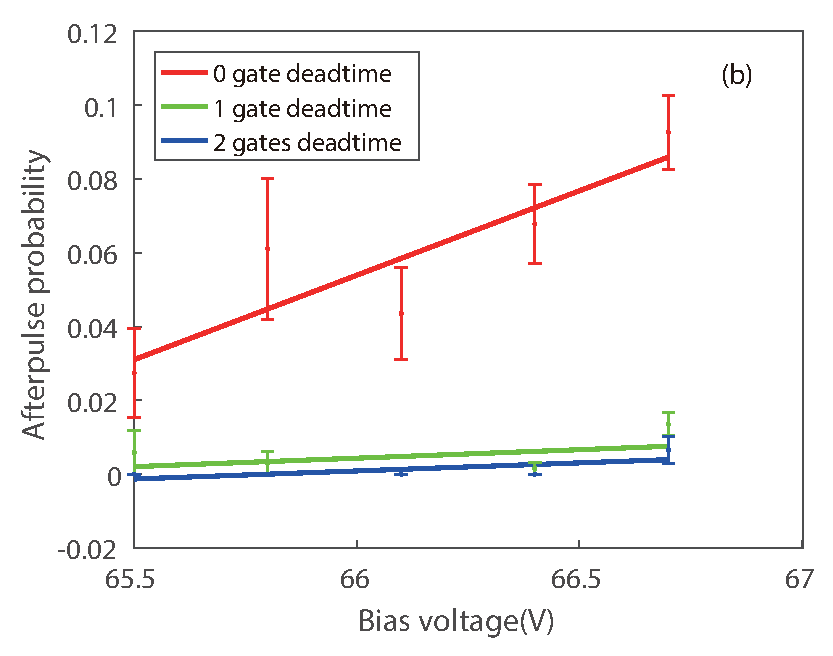
\includegraphics[width = 1\textwidth]{figure/afterpulse_fit.eps}% no-counts-100M-1.2V-66.1V-6-biased
\end{minipage}
\vskip -0.1in
\caption{\label{fig:fit}Specifics at 1000MHz gate repetition frequency with 7.84V peak-peak gate voltage. (a) Detection efficiency and dark count probability, (b) afterpulse probability with 0, 1 and 2 gates of dead time.}
\vskip -0.1in
\end{figure}

\begin{figure}
%begin{tabular}{cc}
\begin{minipage}{0.45\linewidth}
\centering
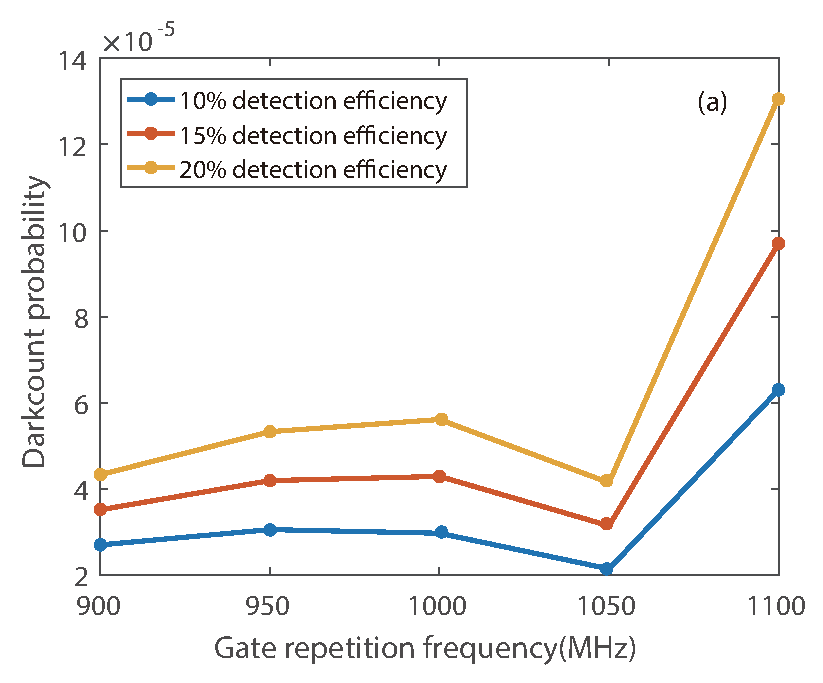
\includegraphics[width = 1\textwidth]{figure/darkcount_rate.eps}% no-counts-100M-1.2V-66.1V-6-biased
\end{minipage}
\begin{minipage}{0.45\linewidth}
\centering
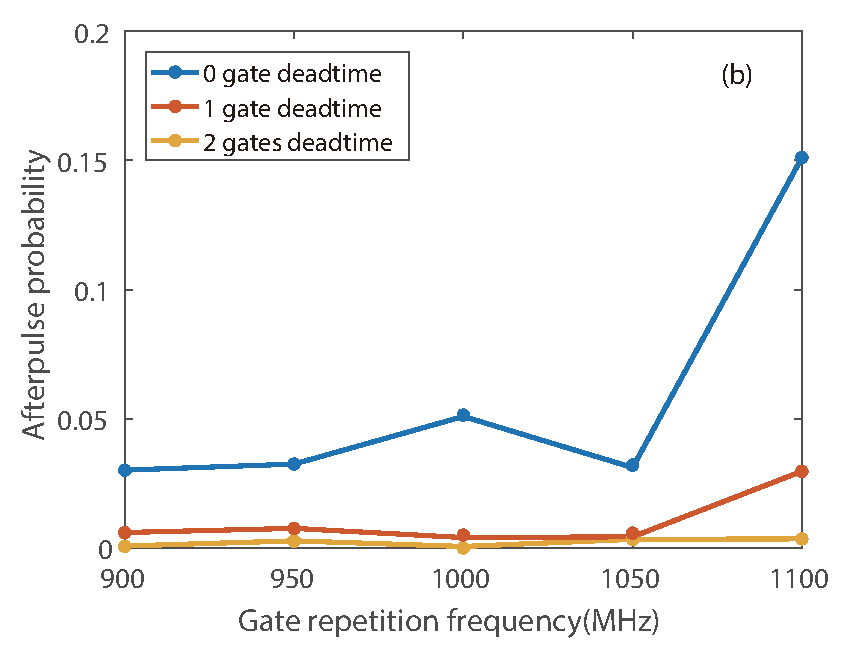
\includegraphics[width = 1\textwidth]{figure/afterpulse_rate_10percent_efficiency.eps}% no-counts-100M-1.2V-66.1V-6-biased
\end{minipage}
\begin{minipage}{0.45\linewidth}
\centering
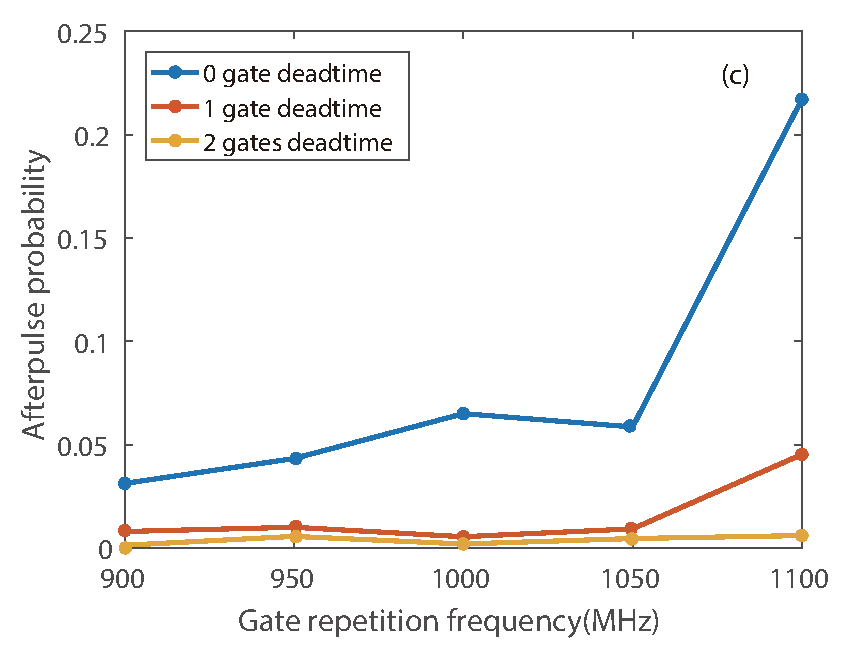
\includegraphics[width = 1\textwidth]{figure/afterpulse_rate_15percent_efficiency.eps}% Here is how to import EPS art
\end{minipage}
\begin{minipage}{0.45\linewidth}
\centering
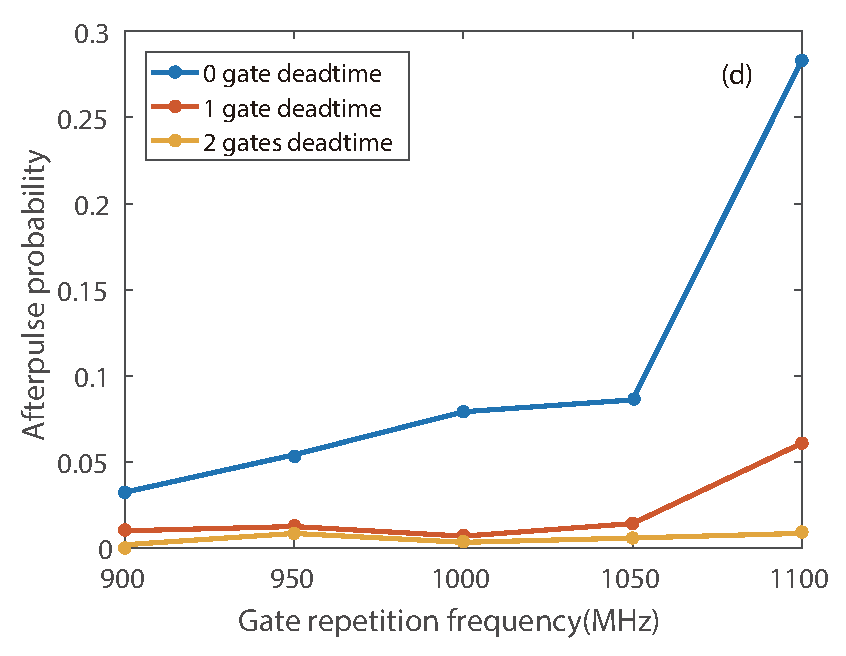
\includegraphics[width = 1\textwidth]{figure/afterpulse_rate_20percent_efficiency.eps}%
\end{minipage}
\vskip -0.05in
\caption{\label{fig:afterpulse_darkcount_rate}(a) Dark count probability at different gate repetition frequency. (b) Afterpulse probability at 10\% detection efficiency. (c) Afterpulse probability at 15\% detection efficiency. (d)  Afterpulse probability at 20\% detection efficiency.}
\vskip -0.2in
\end{figure}

\autoref{fig:afterpulse_darkcount_rate}(a) shows the dark count probability respected to the gate repetition frequency. At 10\% detection efficiency, the dark count probability is around $3\times10^{-5}$. The dark count probability increases with the gate repetition frequency. \autoref{fig:afterpulse_darkcount_rate} (b) shows that the afterpulse probability with no additional gate dead time is quite high, ranging from 3\% to 15\% at 10\% detection efficiency. However, if 1 additional gate software dead time is used, the afterpulse will be greatly decreased to 0.6\% to 3\%. What's more, if 2 additional gate software dead time is used, the afterpulse will be greatly decreased to 0.08\% to 0.35\%. At 15\% detection efficiency and 20 \% detection efficiency also have the same decrease trend as shown in \autoref{fig:afterpulse_darkcount_rate} (c) and \autoref{fig:afterpulse_darkcount_rate} (d).
%
%\begin{figure}
%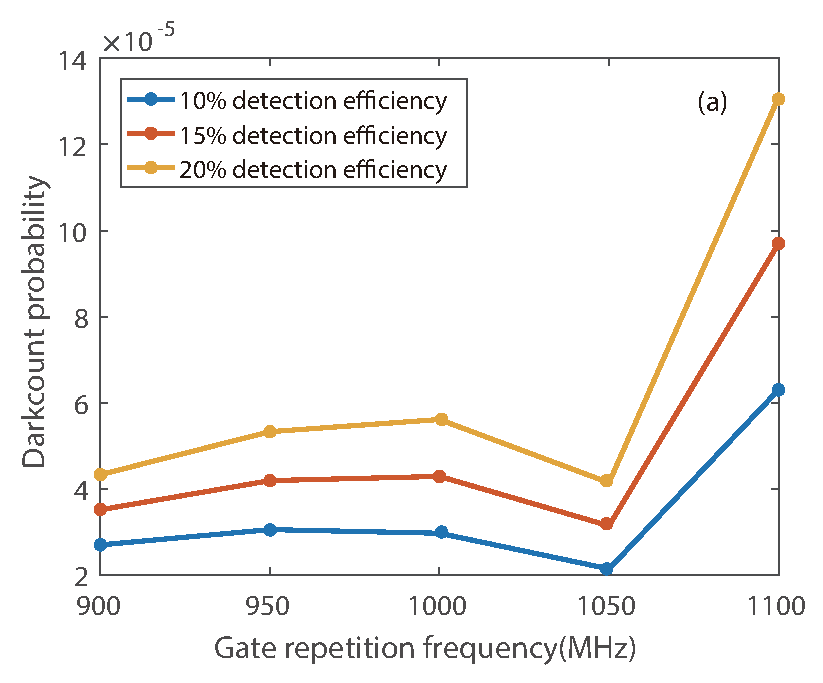
\includegraphics[width = 0.4\textwidth]{figure/darkcount_rate.eps}% Here is how to import EPS art
%\caption{\label{fig:darkcount_rate} Dark count rate at different gate repetition frequency.}
%\end{figure}

Table~\ref{tab:comparison} shows a comparison of our results at 1GHz gate repetition frequency with the other reported high-speed SPDs. At both 10\% and 20\% detection efficiency, we achieves a very low afterpulse probability with 1 additional gate dead time, which means the detection rate can reach as high as 500MHz. Also the dark count probabilities are at the same level with other SPADs which also working at room temperature.

In conclusion, we report a single photon avalanche detector DS-SPD which can work at continuous tunable frequency from 900MHz to 1100MHz at sinusoidal gate mode. An ADC is used to sample the output of the APD without suppressing the response noise. By using this technique, we can discriminate a very weak avalanche signal from the response noise. As a result, a dark count probability of $3\times10^{-5}$ and afterpulse probability  of 0.4\% with 1ns software dead time working at room temperature at 10\% detection efficiency and 1GHz gate repetition frequency was achieved. Furthermore, the circuits of the detector is quite simple and works at room temperature make it very robust and portable. The most important is that the APD can work in high speed at broad frequency of the sinusoidal gate instead of a fixed or narrow frequency used in SD or filtering method. With the tunable gate frequency, the SPAD can be commercially produced and exploited for different and innovative applications.

The authors thank Queentest for providing ADQ7 product. This work is supported by the National Natural Science Foundation of China, Grants No.61072071 and No.11304391. L.-M.L. is supported by the Program for New Century Excellent Talents.
\bibliography{DS-SPD}
\end{document}
%
% ****** End of file apssamp.tex ******
